%%%%%%%%%%%%%%%%%%%%%%%%%%%%%%%%%%%%%%%%%%%%%%%%%%%%%%%%%%%%
% Dokument-Einstellungen
\documentclass{SMBV13}

\setcounter{tocdepth}{5} %to make it appears in TOC
\setcounter{secnumdepth}{5} %to make it numbered

\usepackage{textcomp}
\usepackage{amsmath}
\usepackage{amsthm}
\newtheorem{definition}{Definition}
\newtheorem{theorem}{Theorem}[section]
%\usepackage{algorithm}
%\usepackage{algpseudocode}
%\renewcommand{\algorithmicrequire}{\textbf{Input:}}
%\renewcommand{\algorithmicensure}{\textbf{Output:}}

%%%%%%%%%%%%%%%%%%%%%%%%%%%%%%%%%%%%%%%%%%%%%%%%%%%%%%%%%%%%
%-----------------------------------------------------------
% Hier beginnt das eigentliche Dokument
\begin{document}

\title{Graph-Based Segmentation}

\author{Phan-Anh Nguyen}

\maketitle

%%%%%%%%%%%%%%%%%%%%%%%%%%%%%%%%%%%%%%%%%%%%%%%%%%%%%%%%%%%%
%-----------------------------------------------------------% Zusammenfassung

\begin{abstract}%
The purpose of image segmentation is to partition an image into meaningful regions with respect to a particular application. Segmentation is commonly used in medical image processing to locate tumors, measure tissue volumes and to study anatomical structure. Segmentation is also a crucial part in scene understanding for autonomous systems. However there are several issues often encountered during segmentation. First, the object we want to detect does not always have the same shape. This can cause troubles for the segmentation methods that depend on pre-defined shapes. Secondly, there are no clear boundaries between objects and background due to image clutters and noises. This seminar paper reviews three novel graph-based approaches to the image segmentation problem. The first approach builds a region graph to detect object as the optimal subgraph weighted by a support vector machine classifier applied to bag-of-features regions. The second approach identifies salient contours within an image by solving an Hermitian eigenvalue problem on a contour grouping graph. The third approach extends the min-cut algorithm to solve the multi-class segmentation problem on a Markov random field. Pros and cons and some comparisons between these graph-cut methods are discussed at the end of the present seminar paper.
\end{abstract}

\keywords{Classification, Graph-Cut, Segmentation}

%%%%%%%%%%%%%%%%%%%%%%%%%%%%%%%%%%%%%%%%%%%%%%%%%%%%%%%%%%%%
%-----------------------------------------------------------
%
\section{Introduction}

Image segmentation is an initial and vital step in the whole image processing pipeline aimed at overall image understanding. Segmentation is often used to identify objects in a scene for object-based measurements such as size and shape. This is particularly useful for computer-aided diagnosis applications which assist physicians in finding abnormalities based on medical images of patients. Segmentation is also used to identify obstacles in depth images taken from a mobile robot to generate the optimal path. There are two main problems that prohibit the segmentation task from delivering good results. First, the object we want to detect does not always have the same shape. This can cause troubles for the segmentation methods that depend on pre-defined shapes. Secondly, there are no clear boundaries between objects and background due to image clutters and noises.

Graph-based segmentation is currently emerging as a promising method and has been applied successfully to many image processing applications ranging from scene understanding and segmentation to medical image analysis. Formulating segmentation problems by means of graph theory has a twofold advantage: Firstly, graph representation is an abstract way to encode generic complex relationships between entities, thereby opening up to a wide variety of interpretations for the segmentation problems provided that they can define some metrics to measure the relationships; Secondly, graph representation often leads to well-known graph problems which have been studied for a while and therefore can be solved efficiently.

In general, a graph-based segmentation method often follows the following pipeline. First, image features, which are signal responses from some filters describing important image properties, are extracted from an input image. These features serve as numerical elements used to construct a graph often based on supervised learning algorithms. Once we have built a graph to represent the image segmentation problem, we can apply state-of-the-art graph-cut algorithms to solve the problem efficiently. 

Beside graph-based approaches, a wide variety of segmentation methods have been proposed. Mortensen et al. \cite{mortensen1995intelligent} introduced an interactive segmentation system in which an user picks up some seed points to define a contour that can automatically snap around the object of interest. The system used the Dijkstra's shortest path algorithm to find the lowest cost path in a cost image which is defined based on gradient. Chan and Vese proposed a segmentation method called ``Active contours without edges'' \cite{chan2001active} which used level set formulation to model the evolution of boundaries under internal and external forces. The system did not use gradient for stopping condition thereby being able to identify objects that are very smooth, or even have discontinous boundaries. The system proposed by Fripp et al. \cite{fripp2007automatic} uses three-dimensional active shape models to segment cartilages and rebuild a 3D-model of them. The reconstruction error is below 1 mm.

This seminar paper presents several different graph-based approaches to the image segmentation problem and demonstrates some applications of these techniques to real-world problems. Particularly, Section $\ref{sec:features}$ describes several methods to extract features from images notably Speeded Up Robust Features (SURF) \cite{bay2006surf} is used to describe local image information around a feature point as well as a shape descriptor \cite{gu2009recognition} based on the Globalized Probability of Boundary (gPb) \cite{martin2004learning} \cite{maire2008using}. Section $\ref{sec:supervised_learning}$ introduces some supervised learning techniques which are used in Section $\ref{sec:graph_cunstruction}$ to construct a graph. Section $\ref{sec:graph_cut_algorithms}$ presents powerful graph-cut algorithms used to select optimal subgraphs as segmentation solutions. The applications of graph-cut algorithms to solve the segmentation problem are illustrated in Section $\ref{sec:applications}$ in three different systems namely ``Efficient Region Search'' \cite{VijayGrauman2011} to search for an object of arbitrary shape, ``Contour Cut'' \cite{KenGalShi2011} to identify salient contours in images and ``Multi-Shape Graph-Cut'' \cite{nakagomimulti} to perform lung segmentation based on multiple shape priors. Finally, Section $\ref{sec:conclusion}$ discusses advantages and disadvantages and gives some comparisons between these graph-cut methods.


%%%%%%%%%%%%%%%%%%%%%%%%%%%%%%%%%%%%%%%%%%%%%%%%%%%%%%%%%%%%
%-----------------------------------------------------------
%
\section{Image Features}
\label{sec:features}
Low level image features are essential building blocks for high level image processing tasks such as object detection, image categorization or segmentation. In general, image features capture important properties around local image regions in the form of high dimensional feature vectors that can be used by high level applications. The advantage of the compact representation of features is that it can be readily fed into standard algorithms which often take high dimensional vectors as input. Also features are often made to be invariant to different transformations e.g. rotation, scaling etc. Since features are defined locally, they are invariant to translation. To support real-time systems features need to be efficient to compute. Normally, raw features are extracted at each pixel by applying various kinds of filters. Each filter response corresponds to one dimension in the feature vector space. The shape and size of filters reflect local structure around each pixel. Raw features at each pixel can be collected to form region descriptors which can be used to represent shapes, contours etc. In this section, we present methods to extract raw features and various ways of constructing region descriptors. Specifically, Section $\ref{sec:surf}$ describes a state-of-the-art feature named Speeded Up Robust Features (SURF) \cite{bay2006surf} and Section $\ref{sec:shape_feature}$ explains the Globalized Probability of Boundary (gPb) contour detector \cite{maire2008using}.


%%%%%%%%%%%%%%%%%%%%%%%%%%%%%%%%%%%%%%%%%%%%%%%%%%%%%%%%%%%%
\subsection{Speeded Up Robust Features}
\label{sec:surf}
Speeded Up Robust Features (SURF) \cite{bay2006surf} was originally developed for the task of finding point correspondences between two images of the same scene. This includes three main steps. First, interest points are selected at distinctive locations in the image. Then a feature vector is extracted from the neighbourhood of every interest point. Finally, the feature vectors are matched between different images. Since the SURF descriptor provides a very good representation of a local region it has also been applied to tasks other than correspondence problems such as image classification or image segmentation.

Regarding the interest point detection problem the choice of a detector varies depending on the needs of the application. An application for image registration requires the same interest points to be detected in two different images of the same scene under different viewing conditions. In this case, a detector would pick up hard-to-miss points which appear in both images such as peaks in signal responses corresponding to blobs or corners. In the case of image segmentation it would be a wise choice to select points on contours to be interest points. In the original SURF paper Bay et al. suggested to use an approximate Hessian detector to search in scale-space domain for points having strong derivatives in two orthogonal directions as interest points (often located at corners and strongly textured areas).

Given an interest point in the input image the SURF descriptor is obtained by extracting distinctive information around its neighborhood in a form of a feature vector. The SURF descriptor is designed to be invariant to image scaling and rotation while it can be computed very fast. Scale invariance is achieved by adopting the scale at which the Hessian detector attains maximal response. In order to be invariant to rotation we first find a reproducible orientation based on information within a circular region around the interest point. We then construct a square region aligned to the selected orientation and extract the SURF descriptor from it.

To find the dominant orientation Haar wavelet responses in $x$ and $y$ directions ($d_x$, $d_y$) are calculated within a circular neighbourhood of radius $6s$ around the interest point and weighted with a Gaussian ($\sigma = 2s$), where $s$ is the scale chosen above. Figure $\ref{fig:haar_wavelet}$ shows the structure of the Haar wavelet filters. The wavelet responses ($d_x, d_y$) are then represented in a vector space and the sum of all vectors within a sliding orientation window of size $\frac{\pi}{3}$ is calculated, see Figure $\ref{fig:orientation_window}$. The dominant orientation is finally assigned to the sum vector having the maximal length.

\begin{figure}[htbp]
    \centering
    \subfigure[]
    {
        
\includegraphics[width=0.15\textwidth]{Bilder/SMBV13_EMuster_fig1}
        \label{fig:haar_wavelet}
    }
    \subfigure[]
    {
        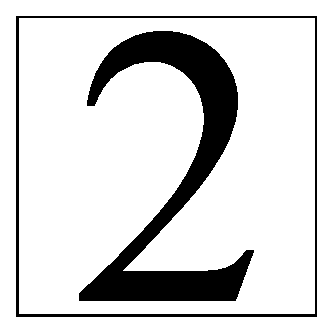
\includegraphics[width=0.25\textwidth]{Bilder/SMBV13_EMuster_fig2}
        \label{fig:orientation_window}
    }
    \subfigure[]
    {
        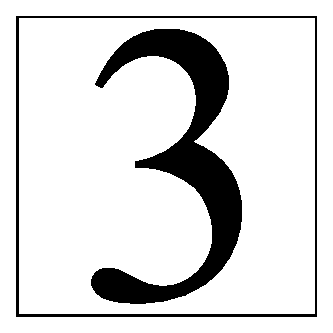
\includegraphics[width=0.5\textwidth]{Bilder/SMBV13_EMuster_fig3}
        \label{fig:surf}
    }
    \caption{(a) Haar wavelet filters for the x (left) and y (right) components. The dark parts are weighted -1 and the light parts +1. (b) Orientation assignment: A sliding orientation window of size $\frac{\pi}{3}$ detects the dominant orientation. (c) The SURF descriptor: An oriented quadratic grid with $4 \times 4$ square cells is laid over the interest point (left). For each cell, the wavelet responses are computed from $5 \times 5$ samples (for illustrative purposes, only $2 \times 2$ sub-divisions are shown here). In each cell, the 4 elements $\sum d_x$, $\sum \left| d_x \right|$, $\sum d_y$, $\sum \left| d_y \right| $ contribute to the SURF feature vector. The images are taken from \cite{bay2006surf}.} 
    %\label{fig:surf}
\end{figure}

To extract the SURF descriptor, we construct a window of size $20s$ centred at the interest point and oriented in the dominant orientation as illustrated in Figure $\ref{fig:surf}$. The window is then subdivided into regular $4 \times 4$ grid cells, each being a $5 \times 5$ pixel patch. For each cell, the Gaussian weighted ($\sigma = 3.3s$) Haar wavelet responses are summed up to form a first set of entries in the feature vector. The sum of the absolute values of the responses, $\left| d_x \right| $ and $\left| d_y \right| $ are also extracted to capture information about the polarity of the intensity changes. Therefore, each cell has a 4D descriptor vector for its underlying intensity structure $\left( \sum d_x, \sum d_y, \sum \left| d_x \right| , \sum \left| d_y \right|  \right)$. Concatenating this for all $4 \times 4$ cells results in a descriptor vector of length 64. Finally the descriptor vector is normalized to make it invariant to contrast.

%%%%%%%%%%%%%%%%%%%%%%%%%%%%%%%%%%%%%%%%%%%%%%%%%%%%%%%%%%%%
\subsection{Globalized Probability of Boundary}
\label{sec:shape_feature}

The globalized probability of boundary (gPb) contour extractor was developed based on the predecessor, namely probability of boundary (Pb), which uses features extracted from a local image patch to estimate the posterior probability of a boundary passing through the current pixel. gPb improves from Pb by introducing global information based on spectral graph theory. In this section we will first survey the local features used by Pb. We will then explain how gPb incorporates global information into Pb. Finally, we will show one method to extract shape descriptors from regions defined by gPb contours. The method to estimate the posterior probability of a boundary will be explained in more detail in Section $\ref{sec:logistic_regression}$.


\subsubsection{Gradient-Based Features for Probability of Boundary}
\label{sec:textons}

The gradient-based paradigm was used by Martin et al. in their $Pb$ paper \cite{martin2004learning} to detect local changes in color, texture and brightness. The algorithm to compute the probability of boundary based on brightness and color features proceeds with the following steps:
\begin{enumerate}
\item At each pixel location $(x, y)$, a circle of radius $r$ is drawn and cut half along the diameter having orientation $\theta$.
\item Histograms of color and brightness in the CIELAB color space \footnote{The CIELAB color space has three dimensions. The L* axis represents lightness ranging from 0 for black to 100 for white. The a* axis is green at one extremity (represented by -a), and red at the other (+a). The b* axis has blue at one end (-b), and yellow (+b) at the other. The color range is between -128 and +127.} are built for each half disk. The L* channel is used to compute the brightness histogram and the a* and b* channels are used to compute the color histogram. 
\item Let $h(x, y, \theta, r)$ and $g(x, y, \theta, r)$ denote the histograms of the two disk halves. We define the gradient function $G(x, y, \theta, r)$ which is the $\chi^2$ distance between the histograms $h$ and $g$:
\begin{equation}
	\chi^2(g, h) = \frac{1}{2} \sum \dfrac{(g_i - h_i)^2}{g_i + h_i}
\end{equation}
\item An edge is detected if there is a large difference $G(x, y, \theta, r)$ between the two half disks along the chosen orientation.
\item A supervised learning method is used to combine the cues into a single detector. This produces soft boundary maps of the form $Pb(x, y, \theta)$.
\end{enumerate}   

\begin{figure}[htbp]
    \centering
    %\subfigure[]
    %{
    %    \includegraphics[width=0.2\textwidth]{images/kde.png}
    %    \label{fig:kde}
    %}
    \subfigure[]
    {
        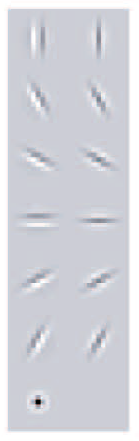
\includegraphics[width=0.1\textwidth]{Bilder/SMBV13_EMuster_fig4}
        \label{fig:filter_bank}
    }
    \subfigure[]
    {
        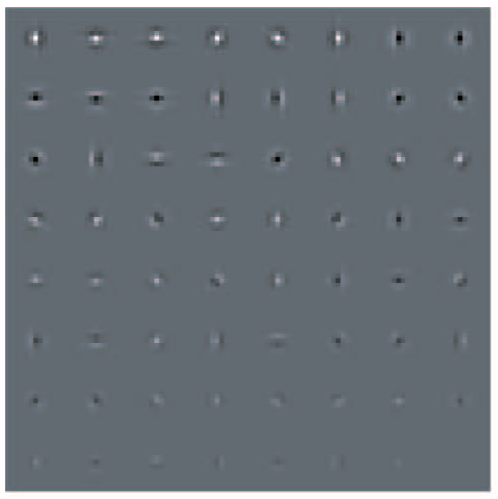
\includegraphics[width=0.3\textwidth]{Bilder/SMBV13_EMuster_fig5}
        \label{fig:textons}
    }
    \subfigure[]
    {
        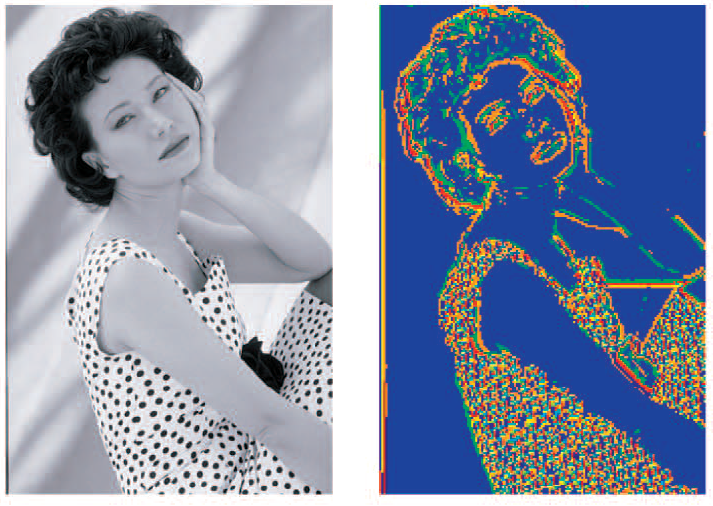
\includegraphics[width=0.5\textwidth]{Bilder/SMBV13_EMuster_fig6}
        \label{fig:texture_map}
    }
    \caption{(a) Filter Bank: The 13-element filter bank used for computing textons. (b) Universal Textons: Example universal textons computed from the 200 training images, sorted by L1 norm for display purposes. (c) Texton Map: An image and its associated texton map. The images are taken from \cite{martin2004learning}.} 
    %\label{fig:texture}
\end{figure}

The same algorithm is used to compute texture gradient but the technique to calculate the texture histogram is different. Specifically, a group of 13 filters covering the most probable shapes is used. It consists of six pairs of elongated, oriented filters and a center-surround filter as shown in Figure $\ref{fig:filter_bank}$. The oriented filters are in even/odd quadrature pairs. The even symmetric filter is a Gaussian second derivative, and the odd-symmetric filter is its Hilbert transform. Finally, a difference of Gaussians is chosen to be the center-surround filter. This filter bank generates a feature vector of 13 dimensions corresponding to 13 filter responses at each pixel.

In order to build up histograms for comparison the $Pb$ algorithm uses the so called textons approach (or bag-of-textures approach) introduced by Malik et al. \cite{malik2001contour}. The basic idea is to cluster the filter response vectors over a large diverse collection of training images using k-means. Each cluster defines a Voronoi cell in the space of joint filter responses and the cluster centers, textons, represent texture primitives. Figure $\ref{fig:textons}$ illustrates example textons for k = 64 computed over the 200 images in the training set. Once the dictionary of textons has been computed each pixel is assigned to the nearest texton. Figure $\ref{fig:texture_map}$ shows an image and the associated texton map, where each pixel has been labeled with the nearest texton. Finally, the histograms of activated textons in the two disc halves can be computed and compared using the $\chi^2$ distance operator.


\subsubsection{Globalized Probability of Boundary Detector}

The gPb contour detector \cite{maire2008using} is an extension of the Pb contour detector into which global information is integrated via spectral graph theory. Particularly, the gPb algorithm follows the idea of the normalized cut algorithm, which defines an affinity matrix $W$, whose entries encode the similarity between pixels. The generalized eigenvectors of the following linear system provide global segmentation information:
\begin{equation}
(D-W)v = \lambda D v
\label{eq:ncut}
\end{equation}
where $D$ is diagonal matrix with $D_{ii} = \sum_j W_{ij}$.
Section $\ref{sec:normalized_cut}$ will explain the normalized cut algorithm in more detail.

We start by extracting the brightness, color and texture gradients in 3 different scales: $[\sigma/2, \sigma, 2\sigma]$, where $\sigma$ is the default scale of the Pb detector. This gives 9 different responses ${G_i}$. These local cues are then linearly combined into a single multiscale oriented signal:

\begin{equation}
mPb(x, y, \theta) = \sum\limits_{i = 1}^{9}\alpha_i G_i(x, y, \theta)
\end{equation}

In order to integrate global information the affinity matrix $W$ is constructed by using the intervening contour cue \cite{leung1998contour}, that is, its entries are the maximal values of $mPb$ along a line connecting two pixels as shown in Figure $\ref{fig:intervening_contour}$. The first $k + 1$ generalized eigenvectors $v_j$ of the system $\ref{eq:ncut}$ are chosen and reshaped in the size of the original image. Contours are extracted from each eigenvector $v_j$ by applying Gaussian directional derivatives at multiple orientations $\theta$, resulting in an oriented signal $sPb_{v_j}(x, y, \theta)$. The information from different eigenvectors is then combined to provide the spectral boundary detector:

\begin{equation}
sPb(x, y, \theta) = \sum\limits_{j=1}^{k}\dfrac{1}{\sqrt{\lambda_j}}sPb_{v_j}(x, y, \theta)
\end{equation}

where $0 = \lambda_0 \leq ... \leq \lambda_k$ are the corresponding eigenvalues. Figure $\ref{fig:sPb}$ illustrates an example of the spectral boundary detector $sPb$.

\begin{figure}[htbp]
    \centering
    \subfigure[]
    {
    	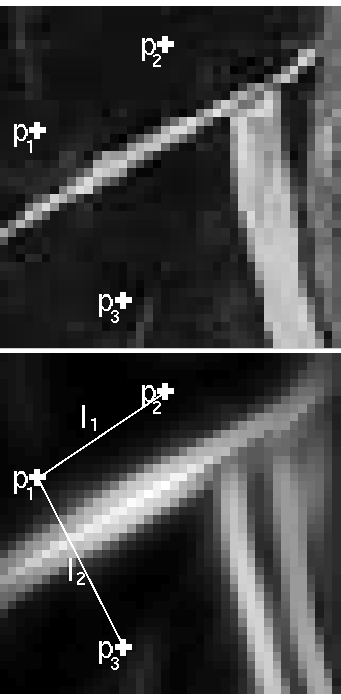
\includegraphics[width=0.15\textwidth]{Bilder/SMBV13_EMuster_fig7}
        \label{fig:intervening_contour}
    }
    \subfigure[]
    {
    	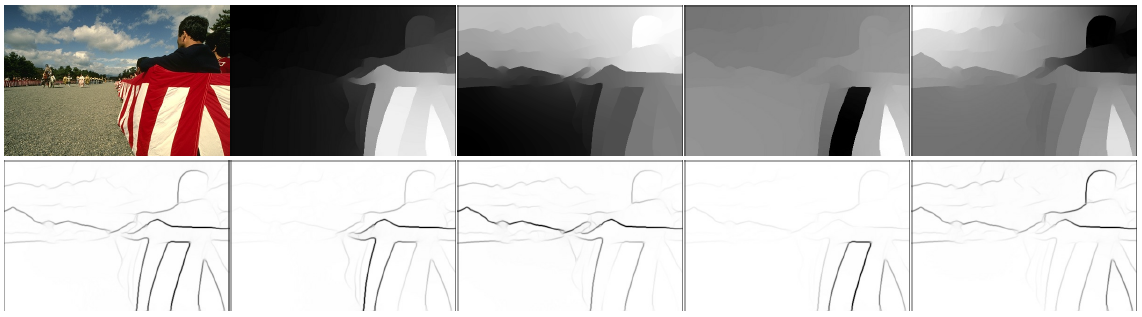
\includegraphics[width=0.8\textwidth]{Bilder/SMBV13_EMuster_fig8}
        \label{fig:sPb}
    }
    \caption{(a) Example of an intervening contour. Above is an image patch in which the intensity values at pixels $p_1, p_2$ and $p_3$ are similar. However, there is an edge in the middle suggesting that $p_1$ and $p_2$ belong to the same group while $p_3$ belongs to a different group. Below is the image computed by using the orientation energy \cite{leung1998contour}. The orientation energy somewhere on $l_2$ is strong which correctly proposes that $p_1$ and $p_3$ belong to two different partitions. (b) Examples from the spectral boundary detector \cite{maire2008using}. Top: Original image and first four generalized eigenvectors. Bottom: Maximum response over orientations $\theta$ of $sPb(x, y, \theta)$ and of $sPb_{v_j}(x, y, \theta)$ for each eigenvector $v_j$.}
\end{figure}

Finally, the globalized probability of boundary , i.e. gPb, is then defined as:

\begin{equation}
gPb(x, y, \theta) = \sum\limits_{i = 1}^{9}\beta_i G_i(x, y, \theta) + \gamma sPb(x, y, \theta)
\end{equation}

where the weights are learned by gradient ascent on the F-measure cost function

\begin{equation}
\mathrm{F} \operatorname{-} \mathrm{measure} = 2\cdot \dfrac{\mathrm{Precision} \cdot \mathrm{Recall}}{\mathrm{Precision + Recall}}.
\end{equation} 


\subsubsection{Shape Descriptor}
\label{sec:shape_descriptor}

The contours detected in the previous section define over-segmented regions of the image. Gu et al. \cite{gu2009recognition} proposed a way to describe a region by evenly subdividing its bounding box into an $n \times n$ grid. The grid size n = 4 has been reported as effective. Each cell encodes information only inside the region. Different cues are extracted from each cell and each type of cue is encoded by concatenating cell signals into a histogram. The following region cues are included:

\begin{itemize}
\item Contour shape, given by the histogram of oriented responses of the contour detector gPb.
\item Edge shape, computed by convolution with a [-1 0 1] filter along x and y axes. This captures high frequency information while it has been smoothed by gPb.
\item Color, represented by the L*, a and b histograms in the CIELAB color space.
\item Texture, described by texton histograms.
\end{itemize}

There are some advantages of this representation, which were pointed out by Gu et al. Firstly, the scale invariant nature of region descriptors enables us to compare regions regardless of their relative sizes. Secondly, background clutter interferes with region representations only mildly compared to interest point descriptors.


%%%%%%%%%%%%%%%%%%%%%%%%%%%%%%%%%%%%%%%%%%%%%%%%%%%%%%%%%%%%
\subsection{Discussion}

So far, we have seen two ways to extract features from an image, each has its own primary purpose. SURF features were originally developed for the problem of image matching but they are also suitable for compact representation of local isotropic image patches. The advantage of using SURF for object detection is its local nature, thereby being invariant to great viewpoint changes having the capability of detecting deformable objects \cite{VijayGrauman2011}. gPb, however, was developed to detect contours, hence being suitable for segmentation tasks \cite{arbelaez2009contours} \cite{gu2009recognition}. It can also be used for part-based object detection \cite{VijayGrauman2011} \cite{gu2009recognition}.

\section{Segmentation with Supervised Training}
\label{sec:supervised_learning}
In image processing, it is very important that algorithms can get some knowledge from the tasks they are going to perform. The knowledge often comes from the training process using pre-defined datasets so that the algorithms can learn from our experiences. This section introduces some supervised learning techniques, that are often used in computer vision tasks.


\subsection{Support Vector Machine}
\label{sec:svm}

The support vector machine (SVM) invented by Cortes and Vapnik \cite{cortes1995support} is a non-probabilistic binary linear classifier, which predicts for each input data point which of the two possible classes the input belongs to. SVM maximizes the margin between positive and negative data points (as shown in Figure $\ref{fig:svm}$), thereby achieving very good generalization performance.

\begin{figure}[htbp]
    \centering
    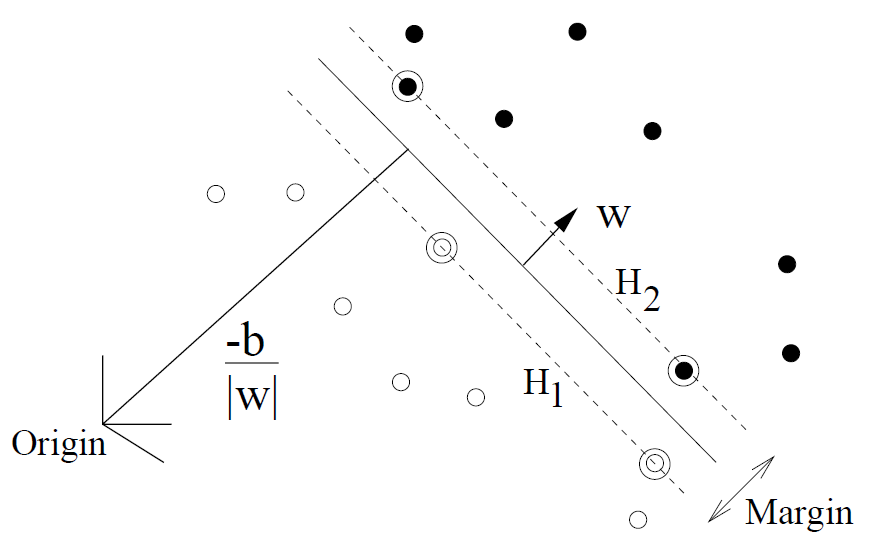
\includegraphics[width=0.60\textwidth]{Bilder/SMBV13_EMuster_fig9}
    \caption{Linear separating hyperplanes for the separable case. The support vectors are circled. Image source: \cite{burges1998tutorial}.}
    \label{fig:svm}
\end{figure}

In this paper we only consider the case of linearly separable data. Suppose we have a dataset of $S$ elements $\left\lbrace (x_i, t_i)\right\rbrace _{i=1}^S$, where $x_i \in R^d$ are training data points with the corresponding target values $t_i \in \left\lbrace -1, 1\right\rbrace $. Our goal is to find a hyperplane of the form $w^T x + b = 0$, which separates the data with maximal margin. The margin is formulated by defining $d_+$ and $d_-$ to be the distances to the nearest positive and negative training examples respectively. We can always scale $w$ and $b$ such that $d_- = d_+ = \dfrac{1}{\|w\|}$. Since the data is linearly separable the separating hyperplane must stay within the following region:
\begin{equation}
t_i(w^T x_i + b) \geq 1\ \forall i
\label{eq:margin}
\end{equation}

The equality in Equation $\ref{eq:margin}$ will hold exactly for the points on the margin. In order to maximize the margin $M = d_- + d_+ = \dfrac{2}{\|w\|}$ we need to minimize $\|w\|$. This can be formally stated as the following optimization problem: find the hyperplane satisfying

\begin{equation}
\operatorname*{arg\,min}_{w, b} \dfrac{1}{2}\|w\|^2
\end{equation}

subject to the constraint in Equation $\ref{eq:margin}$. This quadratic programming problem with linear constraints can be solved efficiently using Lagrange multipliers. The solution for $w$ is obtained as a linear combination of training examples:

\begin{equation}
w = \sum\limits_{i = 1}^{S} a_i t_i x_i = \sum\limits_{i = 1}^{S} \alpha_ix_i,
\end{equation}

where $a_i \geq 0$ is the Lagrange multiplier associate with the training data point $x_i$ and $\alpha_i = a_it_i$. Note that $a_i > 0$ only for training data points on the margin called support vectors. We get the solution for $b$ by observing that any support vector $x_j$ satisfies the equality condition in Equation $\ref{eq:margin}$:

\begin{equation}
\begin{array}{lcl}
t_j \left( \sum\limits_{i = 1}^{S} a_i t_i x_i^t x_j + b \right) = 1\\
b = t_j - \sum\limits_{i = 1}^{S} a_i t_i x_i^t x_j
\end{array}
\end{equation}

In practice, it is more robust to average the solution for $b$ over all support vectors. More detail on extensions to the case of non-separable data as well as non-linear support vector machines can be found in \cite{burges1998tutorial}.


\subsubsection{SVM for Region Ranking}

In this section we will formulate a SVM classifier in a way that it can reliably score a region of arbitrary shape according to how strongly it belongs to a particular object category. It is desirable that features extracted from local image regions can be combined additively to obtain the classifier response for a larger region. It has been proven \cite{lampert2008beyond} that a linear kernel SVM applied to a bag-of-features representation (recall the concept of bag-of-textures from Section $\ref{fig:textons}$) has this additive property. Similar to the textons approach we obtain a vocabulary of K visual words by clustering a sample of local features (e.g. SURF) from the training images. We represent a region by its set of local features $R = \left\lbrace (x_i, v_i) \right\rbrace _{i=1} ^ N$, where $x_i$ is the feature position and $v_i$ the local descriptor. A histogram can be built from this bag-of-features, denoted $h(R)$, by mapping each feature $v_i$ to its closest visual word $d_i$ and recording the frequency of words in a K-dimensional vector.

A linear SVM classifier is learned from the segmented training examples according to the principle described in Section $\ref{sec:svm}$. The region ranking score is then given as follows:
\begin{equation}
\label{eq:svm_classifier}
\begin{array}{lcl}
f(R) & = & b + w \cdot h(R)\\
	 & = & b + (\sum\limits_{i = 1}^{S}\alpha_ih(R_i)) \cdot h(R)\\
     & = & b + \sum\limits_{i = 1}^{K}\sum\limits_{j = 1}^{S} \alpha_ih_j(R_i)h_j(R)\\
     & = & b + \sum\limits_{j = 1}^{K} w_jh_j(R) = b + \sum\limits_{i = 1}^{N} w_{d_i},
\end{array}
\end{equation}
where $d_i \in [1, K]$ is the index of the visual word that feature $v_i$ maps to. Note that we associate each $j$-word in the vocabulary with a weight $w_j = \sum_i \alpha_i h_j(R_i)$ to express $f(R)$ as a sum over per-feature contributions. This means the score of a region is the sum of its N features' word weights. Since we are only interested in maximizing the classifier response $f(R)$ the bias term $b$ is irrelevant and can be ignored.

\subsection{Logistic Regression}
\label{sec:logistic_regression}
In the problem of two-class classification, the logistic regression method models the posterior probability of class $C_1$ by applying a logistic sigmoid function $\sigma$ on a linear discriminant function of the feature vector $\phi$ so that
\begin{equation}
\label{eq:logistic}
\begin{array}{lcl}
	p(C_1|\phi) & = & \sigma(w^T\phi) \\
	p(C_2|\phi) & = & 1 - p(C_1|\phi) 
\end{array}
\end{equation}
where $w$ is the weight vector of the linear discriminant function. The logistic sigmoid function $\sigma$ is given as follows:
\begin{equation}
\label{eq:Bayes}
\sigma(a) = \dfrac{1}{1 + e^{-a}} 
\end{equation}
Suppose we have a training data set $\left\lbrace \phi_n, t_n \right\rbrace_{n = 1}^N$, where $t_n \in \left\lbrace 0, 1 \right\rbrace$, $t = (t_1, ..., t_n)^T$. With $y_n = p(C_1|\phi_n)$ we can write the likelihood as:

\begin{equation}
p(t|w) = \prod\limits_{n = 1}^{N}y_n^{t_n} (1 - y_n)^{1 - t_n}
\end{equation}

The error function is then defined as the negative log-likelihood, which gives the cross-entropy error function in the form

\begin{equation}
E(w) = - \ln p(t|w) = - \sum\limits_{n = 1}^{N} \left( t_n \ln y_n + (1 - t_n) \ln(1 - y_n) \right)
\end{equation}

Our goal is to learn the weight $w$ such that it minimizes the cross-entropy error function. Due to the nonlinearity of the logistic sigmoid function there is no closed-form solution to this optimization problem. Fortunately, this error function is concave, and hence has a unique minimum. Moreover, this error function can be minimized by using the Newton-Raphson iterative optimization scheme, which uses a local quadratic approximation to the log likelihood function. The Newton-Raphson update, for minimizing a function $E(w)$, is given as follows:
\begin{equation}
w^{new} = w^{old} - H^{-1} \nabla E(w)
\label{eq:logistic_update}
\end{equation}
where $H$ is the Hessian matrix, whose entries are the second derivatives of $E(w)$ with respect to the components of $w$. The gradient and Hessian of this error function are given by
\begin{equation}
\nabla E(w) = \sum\limits_{n = 1}^{N}(y_n - t_n) \phi_n %= \Phi^T(y - t)
\end{equation}
\begin{equation}
H = \nabla \nabla E(w) = \sum\limits_{n = 1}^{N} y_n(1 - y_n) \phi_n \phi_n^T %= \Phi^T R \Phi
\end{equation}
Since the Hessian depends on $w$ through $y_n$ we need to apply Equation $\ref{eq:logistic_update}$ iteratively, each time using the new weight vector $w$. Therefore, this algorithm is known as iterative reweighted least squares or IRLS.

\subsection{Statistical Shape Model}
\label{sec:SSM}
To incorporate shape information into the process of segmenting an object in an image Leventon et al. \cite{leventon2000statistical} introduced a statistical shape model in which a prior on shape variation can be computed based on a set of training instances. Specifically, we need $N^d$ samples in a $d$-dimensional image of size $N$ to represent a shape. If we consider each voxel as one dimension, then a shape $u$ is a point in a high dimensional shape space $u \in R^{N^d}$.

Given the training set $T = \left\lbrace u_1, ..., u_n \right\rbrace$, Our goal is to build a shape model over this distribution of surfaces. Since the shapes live in a high dimensional space with a lot of redundant dimension we can reduce the number of dimensions by using Principal Component Analysis (PCA), which only keeps the most relevant shape variances. Under the PCA transformation, a novel shape $u$ can be written as a linear combination of $k$ principal components:
\begin{equation}
u = \sum\limits_{i = 1}^{k} \alpha_k\hat{u}_k,
\end{equation}
where $\alpha_k$ is a weighting coefficient corresponding to the $k$-th principal component $\hat{u}_k$. This means the shape $u$ has been transformed into a $k$-dimensional vector through PCA. Finally, the Gaussian distribution of shapes living in the $k$-dimensional eigen-subspace is estimated resulting in a so-called Statistical Shape Model.

Figure $\ref{fig:shape_training}$ illustrates some training curves used to estimate the shape models of the corpus callosum. The original segmentations are shown as white curves overlaid on the signed-distance map. Figure $\ref{fig:shape_variance}$ shows the means and three primary modes of variance of the shape distribution of the corpus callosum.

\begin{figure}[htbp]
    \centering
    \subfigure[]
    {
    	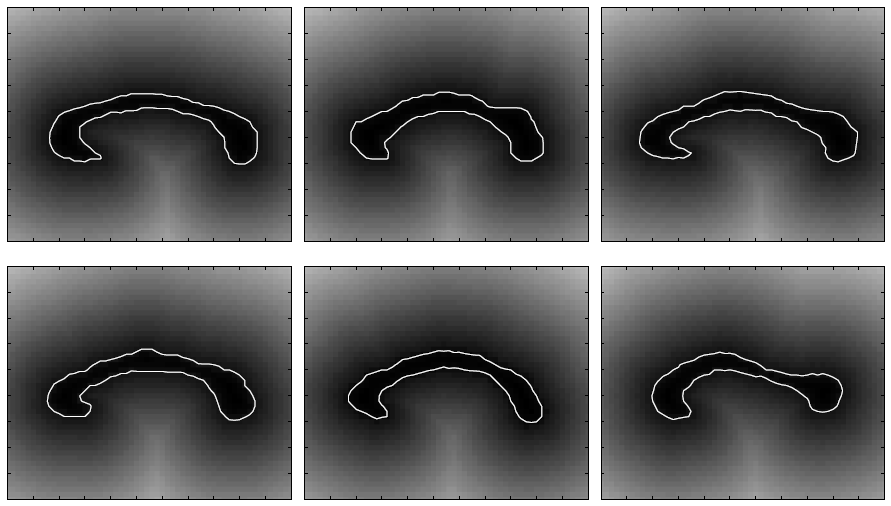
\includegraphics[width=0.45\textwidth]{Bilder/SMBV13_EMuster_fig10}
        \label{fig:shape_training}
    }
    \subfigure[]
    {
    	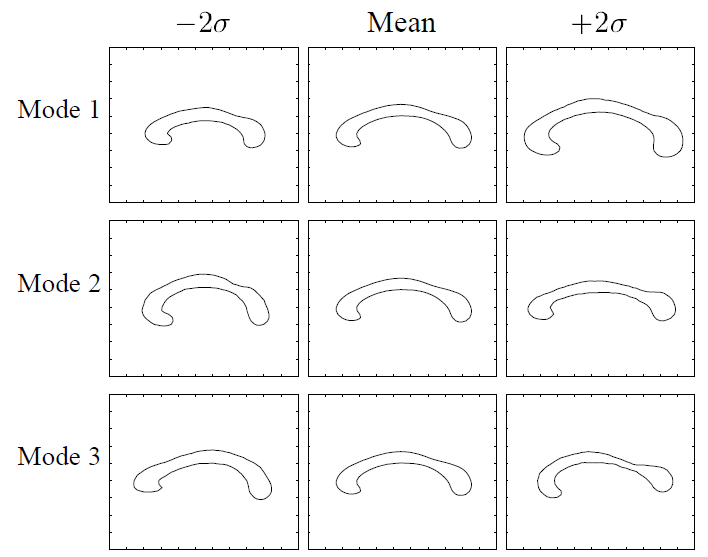
\includegraphics[width=0.45\textwidth]{Bilder/SMBV13_EMuster_fig11}
        \label{fig:shape_variance}
    }
    \caption{(a) some training signed distance maps of Corpus callosum overlaid by the original segmentations. (b) The three primary modes of variance of the corpus callosum training dataset.}
\end{figure}

\section{Graph Construction}
\label{sec:graph_cunstruction}
This section presents three different approaches to construct graphs that represent specific segmentation problems namely region graph for efficient region search problem, contour graph for identifying salient contours and Markov random field for the multi-shape graph-cut problem.
\subsection{Region Graph}
\label{sec:region_graph}
In this section we introduce a method to construct a region graph from an input image, which in turn serves as an input to a graph cut algorithm to find a sub-graph corresponding to the object of interest. This method was proposed by Vijayannarasimhan and Grauman in the object detection context \cite{VijayGrauman2011}. We get the image regions with very high level of detail by applying the oriented watershed transform on the output signal of the gPb contour detector \cite{arbelaez2009contours}. Particularly, a gradient image, which is generated by the gPb contour detector and can be seen as a topographic surface, is pierced at its minima and progressively immersed in water. The water fills the surrounding regions of the minima and forms lakes. When two lakes meet, the level of the water (the height of the saddle point) determines the saliency of the corresponding watershed arc.

The region graph $G = (V, E)$ is built with the set of vertices $V$ being the oversegmented regions, also called superpixels, and the set of edges $E$ connecting any two superpixels that share a boundary. A vertex is weighted with the region ranking formula given in Equation $\ref{eq:svm_classifier}$. Vijayannarasimhan considered two ways to weight a superpixel vertex depending on the type of feature used to construct the histogram $h^v(R)$:

\begin{itemize}
\item Point features: In this representation, each descriptor $v_i$ is a SURF feature and the weight assigned to a superpixel vertex is the sum of the visual word weights for all local features located within that superpixel: $w(v) = \sum_{x_i \in v} w^v_{c_i}$.
\item Shape features: In this case, each superpixel is mapped to a single shape descriptor described in Section $\ref{sec:shape_descriptor}$. Thus, we get the vertex weight $w(v) = w^v_{c_i}$, where $c_i$ is the single visual word associated with that superpixel's shape descriptor.
\end{itemize}

To avoid background regions incorrectly getting included into the result we consider edge weights between pairs of adjacent superpixels based on saliency measures of the wartershed arcs. Since we would like to compute the edge weights by ranking contours within a region just like we did for the vertex weights we introduce a bag-of-contour-strengths histogram vector that captures the statistics of the internal contours within an object. Intuitively, the contours between an object and its background are expected to be highly salient. Therefore, the weights should be learned in such a way that the scores of segmentations, that cross object boundaries, decrease.

Formally, the distribution of contour strengths $h^e(R)$ for an object region $R$ is a histogram of $L$ bins, where each bin represents a given range in the contour saliency measure. Having learned the edge weights $w^e$ as described in the structured SVM learning framework \cite{tsochantaridis2006large}, we can now extend the region ranking score in Equation $\ref{eq:svm_classifier}$ as follows:

\begin{equation}
f^{\prime}(R) = \sum\limits_{i = 1}^{N} w^v_{c_i} - \sum\limits_{j = 1}^{M} w^e_{s_j}
\end{equation}

where $s_j \in [1, L]$ is the bin index of $h^e(R)$ into which the contour strength of the $j^{th}$ contour within the region falls and $M$ denotes the total number of contours in the region $R$. Note that by subtracting the contour term $f^{\prime}(R)$ returns lower scores for regions crossing strong object boundaries, thereby helping to exclude background regions from the optimal solution.

Having constructed a region graph from the input image our goal now is to find a subgraph $R$ maximizing the region ranking score $f^\prime(R)$. The best-scoring subgraph identifies the most likely region for the object of interest. This problem can be transformed into the Prize-Collecting Steiner Tree problem (PCST), which is defined as follows:

\begin{definition}
PCST PROBLEM: Given a connected undirected vertex and edge weighted graph G = (V, E, c, p) with vertex profits $p: V \rightarrow \mathbb{R}^{\geq 0}$ and edge costs $c: E \rightarrow \mathbb{R}^{\geq 0}$, find a connected subgraph T = ($V_T \subseteq V, E_T \subseteq E$) of G that maximizes the profit:
\begin{equation}
P(T) = \sum\limits_{v \in V_T} p(v) - \sum\limits_{e \in E_T} c(e)
\end{equation}
\end{definition}

Note that in the PCST problem both vertex profits and edge costs must be positive while our region ranking scores give both positive and negative values. To circumvent this issue we map $p(v) = w^v(v) - \mu$ and $c(e) = w^e(e) - \mu$, where $\mu$ being the minimum of both vertex and edge weights. The advantage of transforming the region graph into the PCST problem is that we can use a mathematical programming approach, in this case the branch-and-cut algorithm \cite{ljubic2006algorithmic}, to efficiently solve this problem and find the optimal solution. Section $\ref{sec:branch_and_cut}$ discusses this problem in more detail. Figure $\ref{fig:region_graph}$ shows the entire pipeline of this region graph approach.

\begin{figure}[htbp]
    \centering
    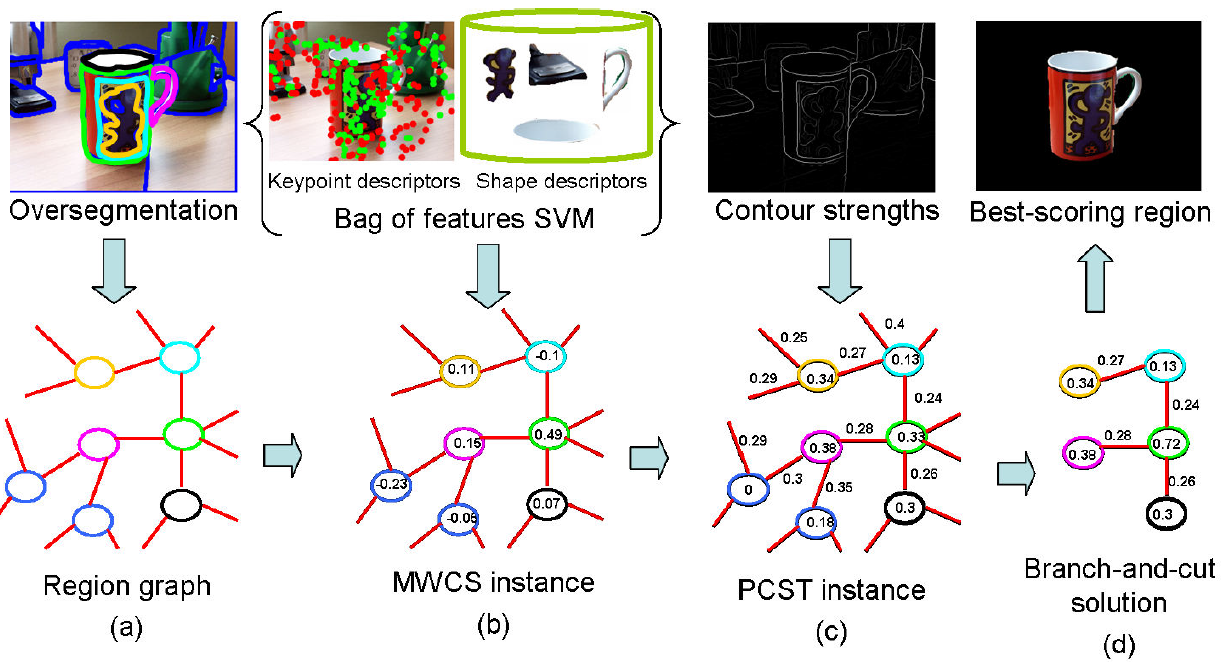
\includegraphics[width=\textwidth]{Bilder/SMBV13_EMuster_fig12}
    \caption{Region graph pipeline. (a) We oversegment the test image and construct a region-graph. (b) A region\textquotesingle s node weight is its contribution to the classifier response. The optimal contiguous set of regions is equivalent to the maximum-weight connected subgraph problem (MWCS) on the vertex weighted region-graph. (c) We incorporate class-specific inter-region contour cues by adding edge costs leading to the PCST problem. (d) The best scoring region is obtained by efficiently solving the PCST instance with a branch-and-cut algorithm. Image source \cite{VijayGrauman2011}.}
    \label{fig:region_graph}
\end{figure}


\subsection{Contour Graph}

In this section, we present a method to construct a directed contour grouping graph \cite{zhu2007untangling} based on which salient contours can be extracted from the otherwise 2D image clutter. Firstly, the output of an edge detector (e.g. gPb) is thresholded to obtain a discrete set of edge segments called edgels. A directed graph $G = (V,E,W)$ is then defined as follows. Graph nodes $V$ correspond to all edgels. Since the edge orientation is ambiguous up to $\pi$, we duplicate every edgel into two copies $i$ and $\bar{i}$ with opposite directions $\theta$ and $\theta + \pi$. Graph edges $E$ include all the pairs of edgels within some distance $r_e$: $E = \left\lbrace (i, j): \| (x_i, y_i) - (x_j, y_j) \| \leq r_e \right\rbrace$. Since every edgel is directed we connect each edgel $i$ only to the neighbors in its direction. Graph weights $W$ measure directed collinearity using the elastic energy between neighboring edgels, which describes how much bending is needed to complete a curve between $i$ and $j$:

\begin{equation}
W_{ij} = e^{-(1 - cos(\mid \phi_i \mid + \mid \phi_j \mid))/\sigma^2}\ \mathrm{if}\ i \rightarrow j
\end{equation}

Here $i \rightarrow j$ means that $j$ is in forward direction of $i$ and $\sigma$ is the scaling factor. $W_{ij} \geq 0$ implies that $W_{ji} = 0$. $\phi_i$ and $\phi_j$ denote the turning angles of $i$ and $j$ w.r.t. the line connecting them as shown in Figure $\ref{fig:contour_graph3}$.

\begin{figure}[htbp]
    \centering
    \subfigure[]
    {
    	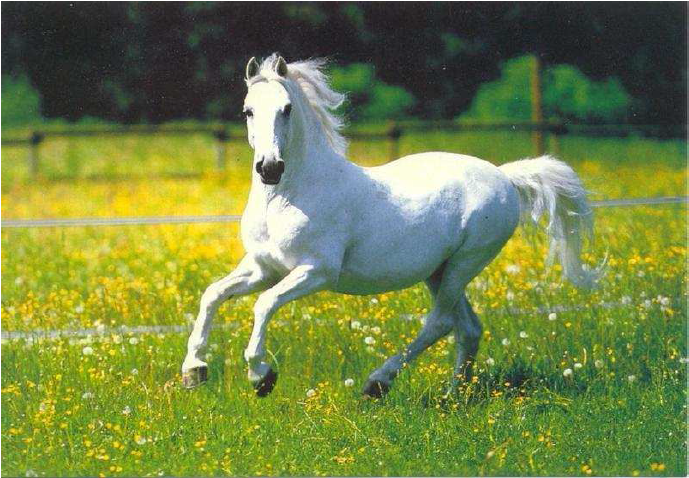
\includegraphics[width=0.23\textwidth]{Bilder/SMBV13_EMuster_fig13}
        \label{fig:contour_graph1}
    }
    \subfigure[]
    {
    	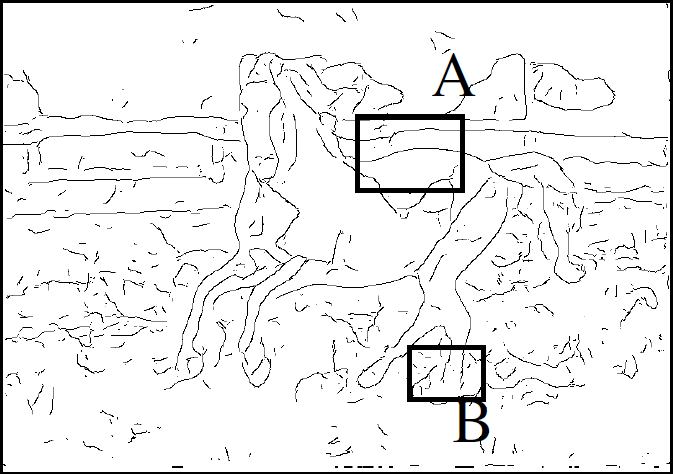
\includegraphics[width=0.23\textwidth]{Bilder/SMBV13_EMuster_fig14}
        \label{fig:contour_graph2}
    }
    \subfigure[]
    {
    	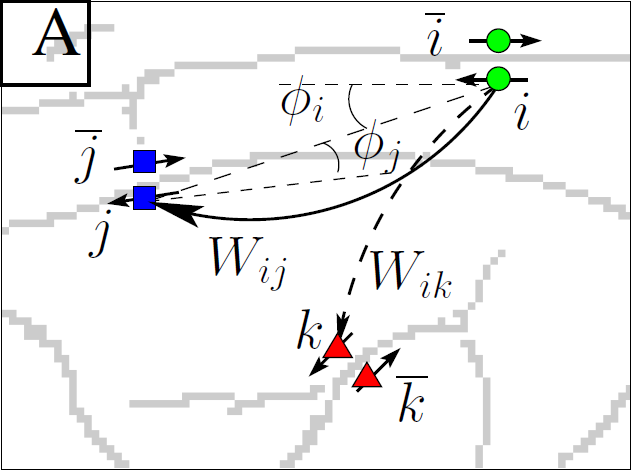
\includegraphics[width=0.23\textwidth]{Bilder/SMBV13_EMuster_fig15}
        \label{fig:contour_graph3}
    }
    \subfigure[]
    {
    	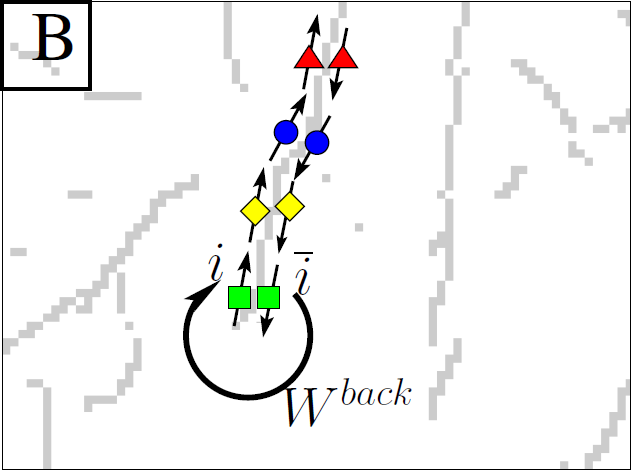
\includegraphics[width=0.23\textwidth]{Bilder/SMBV13_EMuster_fig16}
        \label{fig:contour_graph4}
    }
    \caption{Directed graph for contour grouping. (a) Input image. (b) Edge map extracted from Pb. (c) Zoom-in view of graph connection in window A. Each edge node is duplicated in two opposite orientations. Oriented nodes are connected according to elastic energy and their orientation consistency. Here $W_{ij} \gg W_{ik}$. Salient contours form a 1D topological chain or cycle in this graph. (d) In window B, adding $W^{back}$ to duplicated nodes $i$ and $\bar{i}$ turns a topological chain into a cycle. Image source: \cite{zhu2007untangling}.}
\end{figure}

In this graph, an ideal curve leads to two chains while random clutter produces fragmented clusters in the graph. Our goal is to detect such topological differences and extract 1D topological structures only. To simplify the topological classification task and reduce the search to only cyclic structures we transform two duplicated chains into a cycle by adding a small amount of connection $W^{back}$ between the duplicated nodes $i$ and $\bar{i}$. For open contours, $W^{back}$ connects the termination points back to the opposite direction to create a cycle as illustrated in Figure $\ref{fig:contour_graph4}$.

A contour $(C, O)$ is defined by a set of vertices $C \subseteq V$ and a function $O: C \rightarrow \left\lbrace 1, ..., \lvert C \rvert \right\rbrace$ which specifies a unique ordering of these vertices. To represent a contour $(C, O)$ we must encode nodes which are part of the contour as well as the ordering
of these points. This is accomplished by using a circular embedding where each node of the contour is mapped to a point on a circle about the origin in the complex plane and all other points are mapped to the origin. In this way, each point is represented as complex number
\begin{equation}
x_j = r_j e^{i \theta_j}
\end{equation}
with $r_j = 1$ if $j \in C$ and $0$ otherwise, and $\theta_j = O(j) \delta$ specifies the ordering with $\delta = \frac{2\pi}{\lvert C \rvert}$ is a phase step. The radius $r_j$ of each point encodes whether it is part of the contour.


\subsection{Markov Random Fields}
\label{sec:mrf}
Markov Random Fields (MRF) are undirected graphical models, which formalize and visualize the structure of a probabilistic model through a graph. In MRFs, the nodes correspond to a set of random variables $\left\lbrace x_1, ..., x_n\right\rbrace $, the edges represent soft constraints between them and the graph as a whole can be understood as a joint distribution $p(x)$ over the set of random variables. It is advantageous to express the joint distribution $p(x)$ as a product of functions defined over sets of variables that are local to the graph since this so-called factorized representation conveys interesting information about the properties of the class of distributions that the graph represents. We therefore need to define the appropriate notion of locality through a graphical concept called a clique. A clique is defined as a subset of nodes in a graph such that there exists a link between all pairs of nodes in the subset. In other words, the set of nodes in a clique is fully connected. Furthermore, a maximal clique is a clique such that it is not possible to include any
other nodes from the graph in the set without it ceasing to be a clique. Figure $\ref{fig:clique}$ shows an example of cliques.
\begin{figure}[htbp]
    \centering
    \subfigure[]
    {
    	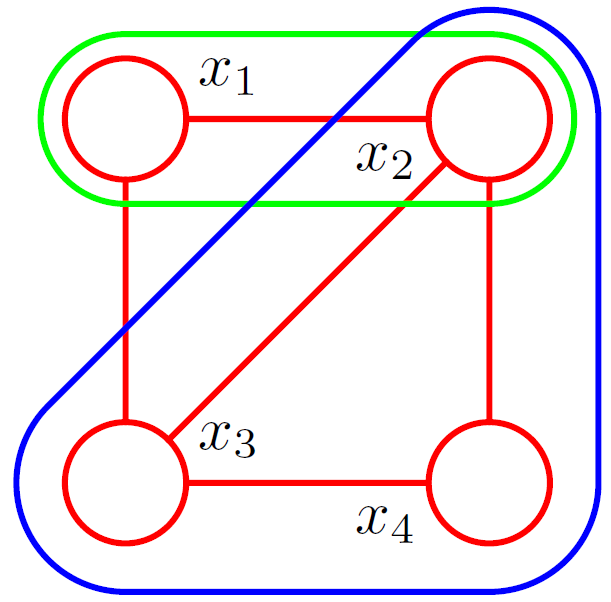
\includegraphics[width=0.2\textwidth]{Bilder/SMBV13_EMuster_fig17}
        \label{fig:clique}
    }
    \subfigure[]
    {
    	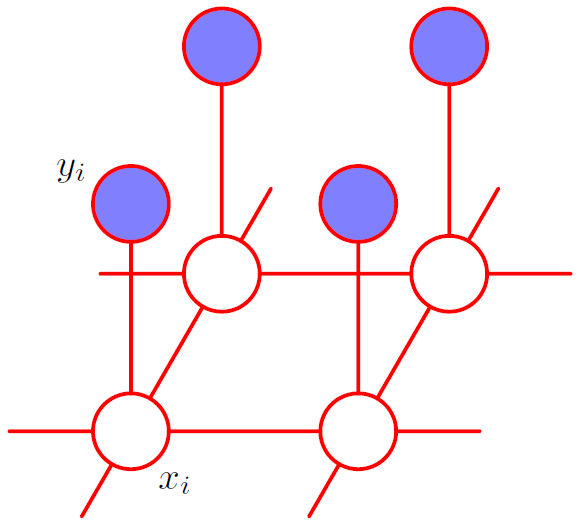
\includegraphics[width=0.25\textwidth]{Bilder/SMBV13_EMuster_fig18}
        \label{fig:mrf}
    }
    \caption{(a) A four-node undirected graph showing a clique (in green) and a maximal clique (in blue). Image source: \cite{bishop2006pattern}. (b) An undirected graphical model representing a Markov random field in which $x_i$ is a variable denoting the hidden true state of pixel $i$ and $y_i$ denotes the corresponding value of pixel $i$ in the observed image data. Image source: \cite{bishop2006pattern}.}
\end{figure}
Given a clique C, we denote the set of variables in that clique by $x_C$. Then the joint distribution is written as a product of potential functions $\psi_C(x_C)$ over the maximal cliques of the graph
\begin{equation}
p(x) = \frac{1}{Z} \prod\limits_{C} \psi_C(x_C)
\label{eq:joint_distribution}
\end{equation}
Here the quantity $Z$, sometimes called the partition function, is a normalization constant and is given by
\begin{equation}
Z = \sum\limits_{x} \prod\limits_{C} \psi_C(x_C)
\end{equation}
which ensures that the distribution $p(x)$ given by Equation $\ref{eq:joint_distribution}$ is correctly normalized. By considering only potential functions, which satisfy $\psi_C(x_C) \geq 0$, we ensure that $p(x) \geq 0$. It is convenient to express $\psi_C(x_C)$ as exponential functions so that
\begin{equation}
\psi_C(x_C) = \exp \left( -E(x_C) \right) 
\end{equation}
where $E(x_C)$ is called an energy function. The joint distribution is defined as the product of potentials and so the total energy is obtained by adding the energies of each of the maximal cliques.

In the field of image processing MRFs are used to capture for each pixel the correlation between the hidden state variable and the observed image data. The spatial coherent of the image content can also be modeled using the neighborhood relationships between pixel state variables as shown in Figure $\ref{fig:mrf}$. 


\subsubsection{Shape Energy}
\begin{figure}
	\centering
    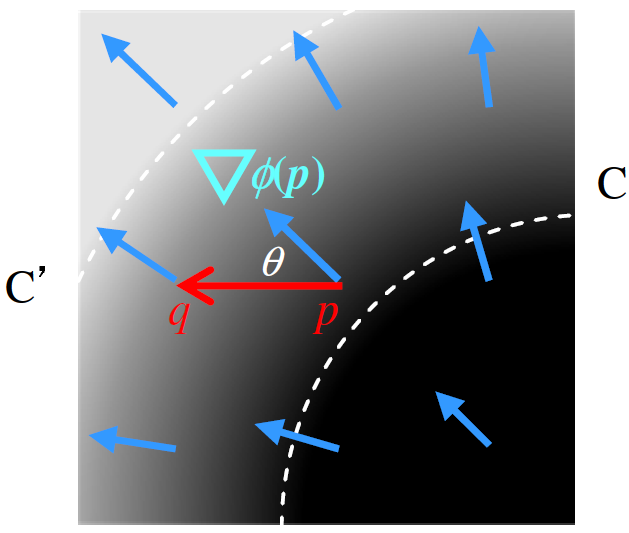
\includegraphics[width=0.3\textwidth]{Bilder/SMBV13_EMuster_fig19}
    \caption{Gradient vectors of $\phi(p)$ and an angle $\theta$ between a gradient vector of $\phi(p)$ and a vector connecting points p and q. Image source: \cite{shimizu2011automated}.}
    \label{fig:shape_energy}
\end{figure}
For the image segmentation problem our goal is to minimize the energy function associated with a MRF constructed from the training data and the observed input image. Particularly, given a set of labels $L = \left\lbrace 0, ..., n \right\rbrace $ we need to find a labelling configuration $A = (A_1, ..., A_{\lvert P \rvert})$ for a set of voxels $P$ that minimizes an energy $E(A)$ given by
\begin{equation}
E(A) = \lambda R(A) + B(A) = \lambda \sum_{p \in P} R_p(A_p) + \sum_{(p, q) \in \mathcal{N}} B_{p, q} \delta_{A_p \neq A_q}
\label{eq:mrf_energy}
\end{equation}
where the set $\mathcal{N}$ is a collection of neighboring voxel pairs, the function $\delta$ is 1 if $A_p \neq A_q$ and 0 otherwise and $\lambda$ is a balancing parameter. There are two types of energy terms in Equation $\ref{eq:mrf_energy}$. The first term $R_p(A_p)$ is a data term which expresses a penalty for assigning label $A_p$ to voxel $p$. Normally, we use the negative log likelihood of the gray value for this term. The second term $B_{p, q}$ is a boundary term which punishes the assignment of labels $A_p$ and $A_q$ to the two neighboring voxels $p$ and $q$. In the context of lung segmentation Shimizu and Nakagomi \cite{shimizu2011automated} \cite{nakagomimulti} proposed a novel energy function incorporating shape energy term $S_{p, q}$ based on multiple shape priors learned with the statistical shape model described in Section $\ref{sec:SSM}$:
\begin{equation}
E(A) = \lambda \sum_{p \in P} \left\lbrace  R_p(A_p) + NB_p(A_p) \right\rbrace + \sum_{(p, q) \in \mathcal{N}} \left\lbrace B_{p, q} + S_{p, q} \right\rbrace \delta_{A_p \neq A_q}
\label{eq:mrf_multishape_energy}
\end{equation}
\begin{equation}
S_{p, q} = \min \left( \sqrt{\dfrac{1 - \cos(\theta_{A_p})}{2}}, \sqrt{\dfrac{1 - \cos(\theta_{A_q})}{2}} \right)
\end{equation}
where $\theta_{A_p}$ represents an angle between a vector connecting voxels $p$ and $q$ and a gradient vector of a signed distance $\phi_{A_p}(p)$ from the boundary of a shape corresponding to a label $A_p \in L$ as shown in Figure $\ref{fig:shape_energy}$. $NB_p(A_p)$ is defined by the distance from the dorsal ribs. This multiple shape MRF problem can be solved using the combination of fusion move and min-cut algorithms explained in Section $\ref{sec:graph_cut}$.


\section{Graph Cut Algorithms}
\label{sec:graph_cut_algorithms}
This part will concentrate on some of the state-of-the-art graph-cut algorithms, which can find a cut that separates the optimal subgraph from those kinds of graphs constructed in Section $\ref{sec:graph_cunstruction}$.

\subsection{Prize-Collecting Steiner Tree}
\label{sec:branch_and_cut}

In this section, we discuss a method to solve the Prize-Collecting Steiner Tree (PCST) problem \cite{ljubic2006algorithmic} of finding a connected subgraph $T = (V_T, E_T)$ that maximizes the profit function defined in Section $\ref{sec:region_graph}$. This maximization problem can be transformed into the problem of finding a subtree $T = (V_T, E_T)$ that minimizes the following function:

\begin{equation}
GW(T) = \sum\limits_{v \notin V_T} p(v) + \sum\limits_{e \in E_T} c(e)
\end{equation}

where $GW(T)$ is the cost function for the subtree $T$. Here, $p(v)$ is interpreted as penalty for not connecting a vertex $v$. Furthermore, we can formulate this problem by means of an integer linear program (ILP) by transforming the reduced graph $G^{\prime} = (V^{\prime}, E^{\prime}, c^{\prime}, p^{\prime})$ resulting from the application of preprocessing into a directed edge-weighted graph $G_{SA} = (V_{SA}, A_{SA}, c^{\prime \prime})$, which is called Steiner arborescence. The vertex set $V_{SA} = V^{\prime} \cup \left\lbrace r \right\rbrace $ contains the vertices of the input graph $G^{\prime}$ and an artificial root vertex $r$. The arc set $A_{SA}$ contains two directed arcs $(i, j)$ and $(j, i)$ for each edge $(i, j) \in E^{\prime}$ plus a set of arcs from the root $r$ to the customer vertices $R_{SA} = \left\lbrace i \in V^{\prime} \lvert p_i^{\prime} > 0 \right\rbrace $, which are the vertices having positive profit. The cost vector $c^{\prime \prime}$ is defined as follows:

\begin{equation}
c_{ij}^{\prime \prime} = 
	\begin{cases} 
		c_{ij}^{\prime} - p_j^{\prime} & \forall (i, j) \in A_{SA}, i \neq r \\ 
		- p_j^{\prime} &  \forall (r, j) \in A_{SA} .
	\end{cases}
\end{equation}

To model the presence or absence of each vertex or edge in the solution $T_{SA}$ we introduce variable vectors $x \in \left\lbrace 0, 1 \right\rbrace ^ {\lvert A_{SA} \rvert}$ and $y \in \left\lbrace 0, 1 \right\rbrace ^ {\lvert V_{SA} \rvert - 1}$ with the following interpretation:

\begin{equation}
x_{ij} = 
	\begin{cases}
		1 & (i, j) \in T_{SA}\\
		0 & \mbox{otherwise}
	\end{cases}
	\forall (i, j) \in A_{SA},\ \ \ 
y_i = 
	\begin{cases}
		1 & i \in T_{SA}\\
		0 & \mbox{otherwise}
	\end{cases}
	\forall i \in V_{SA}, i \neq r.
\end{equation}

Given a set of vertices $S \subset V_{SA}$ and its complement $\bar{S} = V_{SA} \backslash S$ we define two directed cuts: $\delta^+(S) = \left\lbrace (i, j) \lvert i \in S, j \in \bar{S} \right\rbrace $ and $\delta^-(S) = \left\lbrace (i, j) \lvert i \in \bar{S}, j \in S \right\rbrace $. We also write $x(A) = \sum\limits_{ij \in A} x_{ij}$ for any subset of arcs $A \subset A_{SA}$. The corresponding ILP model then reads as follows:

\begin{equation}
\label{eq:ilp_cut}
\mbox{(CUT)} \qquad \min \sum\limits_{ij \in A_{SA}} c_{ij}^{\prime \prime} x_{ij} + \sum\limits_{i \in V_{SA}} p_i^{\prime}
\end{equation}

\begin{equation}
\label{eq:tree}
\mbox{subject to} \qquad \sum\limits_{ji \in A_{SA}} x_{ji} = y_i \qquad \qquad \forall i \in V_{SA} \backslash \left\lbrace r \right\rbrace 
\end{equation}

\begin{equation}
\qquad \qquad \qquad \qquad \qquad x(\delta^-(S)) \geq y_k \qquad \qquad k \in S, r \notin S, \forall S \subset V_{SA}
\label{eq:connectivity}
\end{equation}

\begin{equation}
\sum\limits_{ri \in A_{SA}} x_{ri} = 1
\label{eq:root}
\end{equation}

\begin{equation}
x_{ij}, y_i \in \left\lbrace 0, 1 \right\rbrace \qquad \qquad \qquad \forall (i, j) \in A_{SA}, \forall i \in V_{SA} \backslash \left\lbrace r \right\rbrace 
\end{equation}

Note that the profits from the vertices of the solution have been absorbed into the cost formulation. Therefore, in Equation $\ref{eq:ilp_cut}$ we only penalize those vertices not getting included into the solution. The condition in Equation $\ref{eq:tree}$ is required to ensure a tree structure of the solution. The cut constraints in Equation $\ref{eq:connectivity}$ guarantee that for each vertex $v$ in the solution there must be a directed path from $r$ to $v$. The constraint in Equation $\ref{eq:root}$ is used to ensure the existence and uniqueness of a connection to the root.

In order to create a bijection between arborescence and PCST solutions we introduce the so-called asymmetry
constraints:

\begin{equation}
x_{rj} \leq 1 - y_i, \forall i < j, i \in R
\end{equation}

These inequalities assure that for each PCST solution the customer vertex adjacent to the root is the one with the
smallest index. Note furthermore that in every non-customer vertex, which is not a branching vertex in the Steiner arborescence, the in-degree and the out-degree must be equal, whereas in a branching non-customer vertex the in-degree is always less than the outgoing degree. Thus, we have the following flow-balance constraints:

\begin{equation}
\sum\limits_{ji \in A_{SA}} x_{ji} \leq \sum\limits_{ij \in A_{SA}} x_{ij}, \qquad \forall i \notin R, i \neq r.
\end{equation}

This ILP problem can be solved efficiently in practice with a branch-and-cut algorithm.


\subsubsection{Branch-and-Cut Algorithm}

The branch-and-cut algorithm is a very successful technique for solving a wide variety of integer programming problems to optimality. In essence, it is a combination of a cutting plane method with a branch-and-bound algorithm. These methods work by solving a sequence of linear programming relaxations of the integer programming
problem. Cutting plane methods improve the relaxation of the problem to more closely approximate the integer programming problem and Branch-and-bound algorithms break the problem into sub-problems based on the domain of its variables and proceed by pruning the branches of sub-problems having optimal solutions worse than the bounding value.

We consider a general ILP problem with $n$ variables and $m$ constraints stated as follows

\begin{equation}
\min \left\lbrace c^Tx : Ax \geq b, x \in \mathbb{Z}_+^n \right\rbrace 
\end{equation}

where $x \in \mathbb{Z}_+^n$ is a vector of integer decision variables, $c \in \mathbb{Z}^n$ is the objective function vector, $b \in \mathbb{Z}^m$ is the right hand side vector and $A \in \mathbb{Z}^{m \times n}$ is the matrix of constraint coefficients.

The LP-relaxation (CUT) is obtained by replacing the integrality requirements by their corresponding real-value constraints:

\begin{equation}
\min \left\lbrace c^Tx : Ax \geq b, x \in \mathbb{R}_+^n \right\rbrace 
\end{equation}

Its feasible region is the polyhedron:

\begin{equation}
P = \left\lbrace x \in \mathbb{R}_+^n : Ax \geq b \right\rbrace 
\end{equation}

The integral hull is the convex hull of the set of integer solutions, i.e., the polyhedron:

\begin{equation}
P_I = \mbox{conv} \left\lbrace x \in \mathbb{Z}_+^n : Ax \geq b \right\rbrace 
\end{equation}

We define a cutting plane as a linear inequality that is valid for $P_I$ but not for $P$ as shown in Figure $\ref{fig:cutting_plane}$.
\begin{figure}[htbp]
\centering
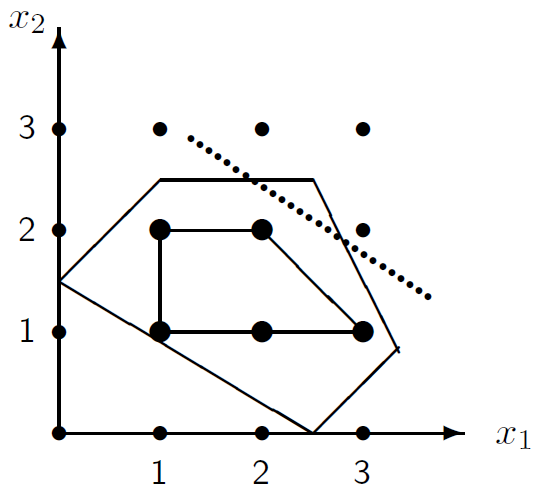
\includegraphics[width=0.3\textwidth]{Bilder/SMBV13_EMuster_fig20}
\label{fig:cutting_plane}
\caption{A cutting plane cuts through the polygon $P$ while trying to get as close to $P_I$ as possible.}
\end{figure}
Following the tutorial of Mitchell \cite{mitchell2002branch} the branch-and-cut algorithm is outlined as follows:

\begin{enumerate}

\item Initialization: Denote the initial integer programming problem by $ILP^0$ and set the active nodes to be $L = \left\lbrace ILP^0 \right\rbrace $. Set the upper bound to be $\bar{z} = + \infty$ and set the lower bound $\underline{z}_l = - \infty$ for the problem $l \in L$.

\item Termination: If $L = \emptyset$, then the solution $x^*$ which yielded the incumbent objective value $\bar{z}$ is optimal. If no such $x^*$ exists (i.e., $\bar{z} = + \infty$) then ILP is infeasible.

\item Problem selection: Select and delete a problem $ILP^l$ from $L$.

\item Relaxation: Solve the linear programming relaxation of $ILP^l$. If the relaxation is infeasible, set $\underline{z}_l = + \infty$ and go to Step 6. Let $\underline{z}_l$ denote the optimal objective value of the relaxation if it is finite and let $x^{lR}$ be an optimal solution; otherwise set $\underline{z}_l = - \infty$.

\item Add cutting planes: If desired, search for cutting planes that are violated by $x^{lR}$; if any are found, add them to the relaxation and return to Step 4.

\item Fathoming and Pruning:

\begin{enumerate}
\item If $\underline{z}_l \geq \bar{z}$ go to Step 2.
\item If $\underline{z}_l < \bar{z}$ and $x^{lR}$ is integral feasible, update $\bar{z} = \underline{z}_l$ , delete from $L$ all problems with $\underline{z}_l \geq \bar{z}$, and go to Step 2.
\end{enumerate}

\item Partitioning: Let $\left\lbrace S^{lj} \right\rbrace _{j = 1} ^ {j = k}$ be a partition of the constraint set $S^l$ of problem $ILP^l$. Add problems $\left\lbrace ILP^{lj} \right\rbrace _{j = 1} ^ {j = k}$ to $L$, where $ILP^{lj}$ is $ILP^l$ with feasible region restricted to $S^{lj}$ and $\underline{z}_{lj}$ for $j = 1, ..., k$ is set to the value of $\underline{z}_l$ for the parent problem $l$. Go to Step 2.

\end{enumerate}


\subsection{Contour Cut}
\label{sec:normalized_cut}
Given a weighted directed graph $G = (V, E, W)$ a random walk on $G$ is a Markov process with transition matrix $P = D^{-1}W$, where $D = \mbox{diag}(\sum_{u}W_{vu})$ is a diagonal matrix with the row-sums of $W$ along the diagonal. Let $\pi$ be the unique left eigenvector such that $\pi P = \pi$. The row-vector $\pi$ corresponds to the stationary distribution of the random walk. This means:
\begin{equation}
\pi_u = \sum\limits_{v, v \rightarrow u} \pi_v P_{vu},
\end{equation}
that is, the probability of finding the random walk at $u$ is the sum of all the incoming probabilities from vertices $v$ that have a directed edges to $u$.

A circulation on a directed graph $G$ is defined as follows.
\begin{definition}
A matrix $F \in (\mathbb{R}^+ \cup \left\lbrace 0 \right\rbrace )^{\lvert V \rvert \times \lvert V \rvert}$ that assigns each directed edge to a non-negative value is called a circulation if
\begin{equation}
\sum\limits_{u, u \rightarrow v} F_{uv} = \sum\limits_{w, v \rightarrow w} F_{vw}
\end{equation}
for each vertex $v$.
\end{definition}
One interpretation of a circulation is a flow in the graph. The flow at each vertex must be conserved, hence, the flow in is equal to the flow out. It is easy to show that $F = \Pi P$ is a circulation in the graph $G$, where $\Pi = \mbox{diag}(\pi)$. This is because the conservation property follows directly from the stationarity property of $\pi$:
\begin{equation}
\sum\limits_{u, u \rightarrow v} F_{uv} = \sum\limits_{u, u \rightarrow v} \pi_u P_{uv} = \pi_v \cdot 1 = \sum\limits_{w, v \rightarrow w} \pi_v P_{vw} = \sum\limits_{w, v \rightarrow w} F_{vw}
\end{equation}
This circulation is advantageous because if $W$ is symmetric then the directed versions of cut and volume that we will define reduce to the original undirected versions \cite{gleich2006hierarchical}.


\subsubsection{Contour Cut Cost}
%\cite{zhu2007untangling}
%\cite{KenGalShi2011}
We define the external cut of a contour $(C, O)$ to measure its separation from the rest of the graph, $V \backslash C$:
\begin{equation}
\mathrm{Ecut}(C) = \sum\limits_{i \in C, j \notin C} F_{ij}
\end{equation}
The internal cut is used to measure the entanglement caused by graph edges within the contour that violate the
ordering $O$. Intuitively, the internal cut measures how much the contour deviates from an ideal one-dimensional contour toward a 2-dimensional clique. Let $k \in \mathbb{Z}^+$ be the width of the contour. Nodes $i, j \in C$ with $\lvert O(i) - O(j) \rvert > k$ are beyond the width of the contour, hence they are included into the internal cut:
\begin{equation}
\mathrm{Icut}(C, O) = \sum\limits_{\left\lbrace i, j\right\rbrace  \subseteq C, \lvert O(i) - O(j) \rvert > k} F_{ij}
\end{equation}
Having defined the external and internal cuts, we can now define the cost function for the contour cut as follows:
\begin{equation}
\mathrm{Ccut}(C, O) = \dfrac{\mathrm{Icut}(C, O) + \mathrm{Ecut}(C)}{\mathrm{Vol}(C)}
\end{equation}
where $\mathrm{Vol}(C) = \sum_{i \in C, j \in E} F_{ij}$ is the sum of the weights of all edges incident with the contour. This cost function will be small for contours having small internal and external cuts.

The internal and external cuts can be encoded with respect to the circular embedding. Given a the circular embedding of a contour, $x \in \mathbb{C}^{\lvert C \rvert}$, the external cut is:
\begin{equation}
\mathrm{Ecut}(x) = \sum\limits_{(i, j) \in E: r_i \neq 0, r_j = 0} F_{ij} = \sum\limits_{(i, j) \in E} F_{ij}r_i(1 - r_j)
\end{equation}
Instead of using the hard-bound of $k$ for the internal cut, a soft version of the internal cut is applied by using the cosine function:
\begin{equation}
\mathrm{Icut}(x) = \sum\limits_{\left\lbrace i, j\right\rbrace \subseteq C}F_{ij} r_ir_j(1 - \cos(\theta_j - \theta_i - \delta))
\end{equation}
The volume of the contour is defined as
\begin{equation}
\mbox{Vol}(x) = \sum\limits_{(i, j) \in E}F_{ij}r_i
\end{equation}
The contour cut in terms of the circular embedding $x$ is then
\begin{equation}
\begin{array}{lcl}
Ccut(x) & = & \dfrac{Icut(x) + Ecut(x)}{\mathrm{Vol}(x)} = ... = \dfrac{x^*(\Pi - H(\delta))x}{x^* \Pi x} = R_{\Pi - H(\delta), \Pi}(x),
\end{array}
\end{equation}
where $H(\delta) = \frac{Fe^{-i\delta} + F^Te^{i\delta}}{2}$ and $R_{\Pi - H(\delta), \Pi}(x)$ is the generalized Rayleigh quotient. It follows that the problem of minimizing $Ccut(x) = R_{\Pi - H(\delta), \Pi}(x)$ is equivalent to maximizing $R_{H(\delta), \Pi}(x)$.




















%%%%%%%%%%%%%%%%%%%%%%%%%%%%%%%%%%%%%%%%%%%%%%%%%%%%%%%%%%%%
%-----------------------------------------------------------
%
\def\refname{Literatur}
\begin{thebibliography}{AA}
                 
\bibitem{mortensen1995intelligent} Mortensen, Eric N., and William A. Barrett: Intelligent scissors for image composition. Proceedings of the 22nd annual conference on Computer graphics and interactive techniques. ACM, 1995.

\bibitem{fripp2007automatic} Fripp, Jurgen and Crozier, Stuart and Warfield, Simon and Ourselin, S{\'e}bastien: Automatic segmentation of articular cartilage in magnetic resonance images of the knee. Medical Image Computing and Computer-Assisted Intervention--MICCAI 2007 (2007): 186--194.

\bibitem{chan2001active} Chan, Tony F and Vese, Luminita A: Active contours without edges. Image Processing, IEEE Transactions on 10.2 (2001): 266--277.

\bibitem{nowozin2009global} Nowozin, Sebastian, and Christoph H. Lampert: Global connectivity potentials for random field models. Computer Vision and Pattern Recognition, 2009. CVPR 2009. IEEE Conference on. IEEE, 2009.

\bibitem{gleich2006hierarchical} Gleich, David: Hierarchical directed spectral graph partitioning. (2006).

\bibitem{lempitsky2010fusion} Lempitsky, Victor, Carsten Rother, Stefan Roth, and Andrew Blake: Fusion moves for markov random field optimization. Pattern Analysis and Machine Intelligence, IEEE Transactions on 32, no. 8 (2010): 1392--1405.

\bibitem{kolmogorov2007minimizing} Kolmogorov, Vladimir, and Carsten Rother: Minimizing nonsubmodular functions with graph cuts-a review. Pattern Analysis and Machine Intelligence, IEEE Transactions on 29.7 (2007): 1274--1279.

\bibitem{boykov2004experimental} Boykov, Yuri, and Vladimir Kolmogorov: An experimental comparison of min-cut/max-flow algorithms for energy minimization in vision. Pattern Analysis and Machine Intelligence, IEEE Transactions on 26.9 (2004): 1124--1137.

\bibitem{mitchell2002branch} Mitchell, John E: Branch-and-cut algorithms for combinatorial optimization problems. Handbook of Applied Optimization (2002): 65--77.

\bibitem{VijayGrauman2011} Vijayanarasimhan, Sudheendra, and Kristen Grauman: Efficient region search for object detection. Computer Vision and Pattern Recognition (CVPR), 2011 IEEE Conference on. IEEE, 2011.

\bibitem{bishop2006pattern} Bishop, Christopher M.: Pattern recognition and machine learning. Vol. 4. No. 4. New York: springer, 2006.

\bibitem{shimizu2011automated} Shimizu, Akinobu, Keita Nakagomi, Takuya Narihira, Hidefumi Kobatake, Shigeru Nawano, Kenji Shinozaki, Koich Ishizu, and Kaori Togashi: Automated segmentation of 3D CT images based on statistical atlas and graph cuts. Medical Computer Vision. Recognition Techniques and Applications in Medical Imaging (2011): 214--223.

\bibitem{KenGalShi2011} Kennedy, Ryan, Jean Gallier, and Jianbo Shi: Contour cut: identifying salient contours in images by solving a Hermitian eigenvalue problem. In Computer Vision and Pattern Recognition (CVPR), 2011 IEEE Conference on, pp. 2065--2072. IEEE, 2011.

\bibitem{nakagomimulti} Nakagomi, Keita, Akinobu Shimizu, Hidefumi Kobatake, Masahiro Yakami, Koji Fujimoto, and Kaori Togashi: Multi-shape graph-cuts and its application to lung segmentation from a chest CT volume.

\bibitem{leventon2000statistical} Leventon, Michael E., W. Eric L. Grimson, and Olivier Faugeras: Statistical shape influence in geodesic active contours. In Computer Vision and Pattern Recognition, 2000. Proceedings. IEEE Conference on, vol. 1, pp. 316--323. IEEE, 2000.

\bibitem{tsochantaridis2006large} Tsochantaridis, Ioannis, Thorsten Joachims, Thomas Hofmann, and Yasemin Altun: Large margin methods for structured and interdependent output variables. Journal of Machine Learning Research 6, no. 2 (2006): 1453.

\bibitem{maire2008using} Maire, M. and Arbel{\'a}ez, P. and Fowlkes, C. and Malik, J.: Using contours to detect and localize junctions in natural images. In Computer Vision and Pattern Recognition, 2008. CVPR 2008. IEEE Conference on, pp. 1--8. IEEE, 2008.

\bibitem{gu2009recognition} Gu, C. and Lim, J.J. and Arbel{\'a}ez, P. and Malik, J.: Recognition using regions. In Computer Vision and Pattern Recognition, 2009. CVPR 2009. IEEE Conference on, pp. 1030--1037. IEEE, 2009.

\bibitem{bay2006surf} Bay, Herbert, Tinne Tuytelaars, and Luc Van Gool: Surf: Speeded up robust features. Computer Vision--ECCV 2006 (2006): 404--417.

\bibitem{ljubic2006algorithmic} Ljubi{\'c}, I. and Weiskircher, R. and Pferschy, U. and Klau, G.W. and Mutzel, P. and Fischetti, M.: An algorithmic framework for the exact solution of the prize--collecting Steiner tree problem. Mathematical Programming 105, no. 2 (2006): 427--449.

\bibitem{shi2000normalized} Shi, Jianbo, and Jitendra Malik: Normalized cuts and image segmentation. Pattern Analysis and Machine Intelligence, IEEE Transactions on 22, no. 8 (2000): 888--905.

\bibitem{zhu2007untangling} Zhu, Qihui, Gang Song, and Jianbo Shi: Untangling cycles for contour grouping. In Computer Vision, 2007. ICCV 2007. IEEE 11th International Conference on, pp. 1--8. IEEE, 2007.

\bibitem{martin2004learning} Martin, David R., Charless C. Fowlkes, and Jitendra Malik: Learning to detect natural image boundaries using local brightness, color, and texture cues. Pattern Analysis and Machine Intelligence, IEEE Transactions on 26, no. 5 (2004): 530--549.

\bibitem{arbelaez2009contours} Arbel{\'a}ez, P. and Maire, M. and Fowlkes, C. and Malik, J.: From contours to regions: An empirical evaluation. In Computer Vision and Pattern Recognition, 2009. CVPR 2009. IEEE Conference on, pp. 2294--2301. IEEE, 2009.

\bibitem{malik2001contour} Malik, Jitendra, Serge Belongie, Thomas Leung, and Jianbo Shi: Contour and texture analysis for image segmentation. International Journal of Computer Vision 43, no. 1 (2001): 7--27.

\bibitem{leung1998contour} Leung, Thomas, and Jitendra Malik: Contour continuity in region based image segmentation. Computer Vision--ECCV'98 (1998): 544--559.

\bibitem{cortes1995support} Cortes, Corinna, and Vladimir Vapnik: Support--vector networks. Machine learning 20, no. 3 (1995): 273--297.

\bibitem{burges1998tutorial} Burges, Christopher JC: A tutorial on support vector machines for pattern recognition. Data mining and knowledge discovery 2, no. 2 (1998): 121--167.

\bibitem{lampert2008beyond} Lampert, Christoph H., Matthew B. Blaschko, and Thomas Hofmann: Beyond sliding windows: Object localization by efficient subwindow search. In Computer Vision and Pattern Recognition, 2008. CVPR 2008. IEEE Conference on, pp. 1--8. IEEE, 2008.

\end{thebibliography}

%\noindent
%\begin{picture}(160,242)
%\put(0,0){\framebox(160,242){}}
%\end{picture}

\end{document}
